\documentclass[11pt]{article}
\usepackage[margin=1.0in]{geometry}
\usepackage{graphicx}
\usepackage[pdftex]{hyperref}
\usepackage{wrapfig}
\usepackage{float}
\usepackage{enumitem}
\usepackage{textcomp}

\title{User Empathy Reflection}
\author{Jonathan "Sumner" Evans}
\date{\today}

\begin{document}
\begin{titlepage}
    \centering
    \vspace{5cm}
    {\huge\bfseries User Empathy Reflection \par}
    \vspace{1cm}
    {\scshape\Large Jonathan "Sumner" Evans\par}
    \vfill
    {\scshape\large Section U\par}
    {\large \today\par}
    \vfill
\end{titlepage}

\section{Introduction}
The goal of our User Empathy Experience was to put ourselves into a situation where we could gain a
deeper understanding of the struggles of people who are living in food deserts and whose primary
monetary resource for purchasing food is the USDA's Supplemental Nutrition Assistance Program
(SNAP) \cite{usda-snap}. To do this, we used public transportation to visit a food desert and obtain
enough food that everyone on the team can eat and enjoy a meal together.

Food deserts are areas where residents have limited access to grocery stores within convenient
traveling distance \cite{fep}. Because of the limited access to these food retailers in food
deserts, access to affordable fruits, vegetables, whole grains, low-fat milk, and other foods that
make up the full range of a healthy diet is limited \cite{cdc}. In many cases, the people living
within the food desert do not own cars \cite{usda-access} further limiting their access to healthy
food options.

SNAP is a USDA program which provides food assistance for low-income individuals and families
\cite{usda-snap}. SNAP provides approximately \$4.32 per person per day to its beneficiaries
\cite{cbpp}. For a family of five, that works out to be \$21.15 for the entire family for the day.
Since my team consists of five members, we also held ourselves to the \$21.15 limit for our Empathy
Experience.

Our goal was to follow the USDA's nutrition recommendations found on
\url{https://www.choosemyplate.gov/} when choosing the food for our meal. According to this website,
if we were buying food for a whole day, we would need the following quantities of each food type for
each person \cite{myplate}:

\begin{itemize}[noitemsep]
    \item $2$ cups fruit
    \item $3$ cups vegetables
    \item $8$ oz equivalents grain
    \item $6\frac{1}{2}$ oz equivalents protein
    \item $3$ cups dairy
\end{itemize}

Since we were only buying food for one meal, the actual quantities would be different, but the
proportions would be approximately the same.

\section{Anticipated Bugs}
Before embarking on the User Empathy Experience with my team, I compiled a list of "bugs" that I
anticipated my team would encounter while in the food desert. Below is that list with an explanation
of each item:

\begin{itemize}
    \item \textbf{Difficulty finding enough fruits and vegetables.} Because food deserts are
        characterized by a lack of affordable fruits and vegetables, I anticipated that it would be
        difficult for my team to find enough fruits and vegetables.

    \item \textbf{Difficulty staying under the SNAP budget.} I anticipated that we would have
        problems staying under the self-imposed SNAP budget. I made this judgment by looking at the
        receipt from a recent grocery trip where my family spent about \$177.00. Dividing this
        number out between the four people in my family results in about \$69.00 per person. \$69.00
        divided by \$4.32 is about $16$ meaning that we would have had to live solely off of the
        food we bought during that shopping trip for $16$ days. In my family, it is common to buy
        groceries once a week, so our changes to our eating habits would be required in order for us
        to consume the proper amount of each food category.

    \item \textbf{Difficulty finding low-fat protein sources.} In many food deserts, fast food
        chains and convenience stores are the closest, if not only, food retailers in the area
        \cite{gallagher}. Although many of these food retailers serve forms of protein, they are
        often high in fat content. Because of this, I anticipated that it would be difficult to find
        low-fat protein sources.

    \item \textbf{Difficulty finding low-fat dairy.} Judging from my past experiences at gas station
        curb stores, high-fat dairy such as ice cream is in abundance, but low-fat dairy such as
        milk or yogurt is not as common. Since curb stores are often the only retailers of food in
        food deserts, I anticipated that it would be difficult to find such low-fat dairy.

    \item \textbf{Difficulties using public transportation.} I have used public transportation in
        many places around the world with varying degrees of success. In some cases, such as when I
        used the Tube in London, things went smoothly. Other cases, such as when I attempted to ride
        a bus in New York City, were not so successful. Despite having grown up in the Denver Metro
        area, I am not very experienced in using the public transportation so I decided to assume
        the worst case scenario. Judging from past mistakes while using public transportation, I
        thought that it would be likely that we might miss the bus, get on the wrong bus, have to
        wait a long time for the bus, or miss a connection with the Light Rail.

        In addition, I expected that it might be cumbersome carrying the groceries on public
        transportation. While in Boston for vacation this summer, I used the public transportation
        system to get around the city and I was often carrying a backpack. This was rather
        cumbersome at times, therefore I expected carrying groceries to also be cumbersome.

    \item \textbf{Significant amount of time to find proper foods} I anticipated that it would take
        a significant amount of time to find the proper foods (if we were even able do to) because
        of all of the aforementioned factors.
\end{itemize}

\section{Actual Bugs}
During my teams trip to our assigned food desert, we encountered many difficulties. Some were
expected, but others were surprising. All of them gave me insight into the difficulties faced by
people living in food deserts.

\begin{itemize}
    \item \textbf{Public transportation issues.} During my team's User Empathy Experience, we
        used three types of public transportation: Light Rail, bus, and walking. We didn't fully
        succeed at any of them. The Light Rail trip from Golden to Wadsworth was uneventful. While
        on the train, I took a picture of the light rail and later sketched it [Fig. 1]. Our
        troubles began after we arrived at the Wadsworth station because we had mistimed our ride
        and the Wadsworth bus was not going to come for another forty-five minutes. We ended up
        walking one mile from Colfax to 26th Avenue. By the time we had walked this distance, the
        bus had caught up to us and we took it from 26th to 38th. Had we waited for the bus to come
        to the Colfax stop, we would have arrived at the same time, without the mile of walking.

        In our food desert, there were some stretches with nice paved sidewalks, but in other
        places the sidewalks were either in poor condition or nonexistent. For example, along
        Wadsworth near the Morning Side Retirement Community, there is no paved sidewalk, it is
        merely trampled down grass and dirt. I thought that it would be difficult for some of the
        less mobile residents of the retirement community to go to the store if that was the only
        sidewalk. When I returned on my own last Friday, I found that there are sidewalks on the
        other side of the retirement community that are in good condition, but when we were there as
        a team, we didn't find those sidewalks.

        After our time in the food desert, we mistimed the bus and ended up walking $1.5$ miles from
        the food desert to the Light Rail stop at Colfax. The bus passed us about a block before we
        got to the Colfax station. As we were coming up to the Light Rail station, we saw the train
        leaving the station so we had to wait for the next train. While we were waiting, we took our
        team photo [Fig. 2].

        As we walked back to the Light Rail station, I was carrying the bag of groceries. Though not
        very heavy, it seemed as though the bag's weight increased with the distance walked. I have
        much more sympathy for people who must carry groceries long distances after having done it
        myself.

        Overall, we were not successful in our use of public transportation. Overall, however, using
        public transportation gave me a greater appreciation for people who rely on public
        transportation for all of their transportation needs.

    \item \textbf{Difficulty finding quality fruits and vegetables.} We bought our food at the
        Shell curb store at 38th and Wadsworth. We found a great lack of fruits and vegetables in
        this location. There were no fresh fruits or vegetables in the store when we went as a team.
        There was a stand for bananas, but it was empty [Fig. 3]. When I returned on my own to the
        food desert, there was one banana in the stand. There was no shortage of fruit-flavored
        candies in the store, but no actual fruit. While at the curb store as a team, the closest
        food product to a fruit that we were able to find was a jar of grape jam, a highly processed
        derivative of a fruit. I knew that it would be difficult to find fruits and vegetables, but
        I was surprised at how sparse the selection was. I expected that there might be some apples
        or bananas consistently available for purchase but after two visits to the curb store, it

        was clear that this was not the case.

    \item \textbf{Difficulty finding low-fat protein.} Like fruits and vegetables, protein was not
        in abundance at the Shell curb store. There were packages of beef jerkey, but they were
        relatively expensive and high in sodium. There were also some nuts, but those, too, were
        high in sodium. We ended up settling for a jar of peanut butter which is high in protein,
        but also fairly high in fat content.

    \item \textbf{Difficulty transporting perishables.} For our dairy product, we purchased some
        milk but did not account for the fact that it needed to be refrigerated. By the time we got
        back to the Mines Campus, the milk noticeably warmer. If the temperature that day had been
        any warmer, or if we had waited longer to prepare our food upon our return to campus, the
        milk may have been warmer and less safe.

    \item \textbf{Possible language barriers.} Our team's food desert was in a mixed-ethnicity
        neighborhood. Much of the area, especially the stretch along the south side of 38th Ave
        seemed predominately White. At 32nd and Wadsworth, there was a small shopping center with an
        Italian bakery and a store which sold products primarily from Eastern Europe. Right next to
        those stores was a Tax Services office which had their services listed in Spanish on the
        windows. Slightly south of the gas station was a Hispanic \textit{jover\'{i}a}, jewelry
        store. The fact there was signage in both English and Spanish, the existence of language
        barriers is likely.
\end{itemize}

\section{Analysis}
\subsection{Demographics}
On our initial visit to the food desert as a team, we did not see many people. We wandered around
inside the curb store for quite some time, but only two or three other people came in. None of the
guests, except the lady who came in wearing a bikini, stood out to me in any way. The employee at

the gas station looked Hispanic. It appeared that he was either very shy or that he was
uncomfortable speaking English because when I tried to ask him some questions about the types of
people who come to the curb store, the only response I received was a mumble and the price of our
food.

As we walked around the food desert area, we saw a very few people. We saw a Hispanic man working on
his yard and we saw a group of teenagers. I do not recall the exact ethnic makeup of this group, but
I do recall at least some of them looked Hispanic.

I felt like I didn't have sufficient time to experience the area when I went with my group so I
returned to the food desert on Friday, 9 September 2016. This time, I drove my car up to the food
desert and drove the perimeter. I also drove about 8 miles through the streets within the food
desert. On this trip, I saw a few more people. There were a few people walking around. I ended up at
the retirement community by accident and saw an older man walking in the area. There were also some
people holding what appeared to be a garage sale. The people at the garage sale appeared to be
middle-aged White people primarily. (I did not want to stare or appear like I was stalking, so I
only had a short glance at the people there.) I also saw a father and his two sons walking home from
school. The father was very overweight but his children seemed average weight and height for their
age.

On this second trip, I stopped at the small shopping center on 32nd and Wadsworth where, as I
described above, there were a variety of stores catering to immigrant populations. The lady working
at the Euro Market Delicatessen looked like she could have been Eastern European herself. I
talked to the lady in the Italian bakery to see if she knew of any major immigrant populations in
the area. She did not seem familiar with the food desert area and was unable to give me any
information. Before leaving the shopping strip, I took a picture of the Euro Market Delicatessen
storefront [Fig. 4].

As I drove around the neighborhood, one thing I noticed was that there were apartments intermingled
with homes. Overall, these homes seemed well kept up. Almost all of the houses had green-grass lawns
and the houses were in good condition. Most of the houses as well as the apartments looked like they
were built in the '60s. I took a picture of one of the apartments and later sketched the apartment
[Fig. 5].

Overall, the neighborhood seemed much more mixed than my own. Whereas I rarely see anyone who is not
White in my neighborhood, probably only $80\%$ of the people in people I saw were White.

\subsection{Food Quality}
As described above, the Shell curb store had no good fruit or vegetable options except that one
banana on my second trip. Of the three and a half isles with food displays, three full isles had
junk food such as candy, chips, and cookies leaving only one isle with actual food.

One interesting thing about the bananas, they were right next to the ice cream freezer. While the
banana stand was not very well stocked, there were plenty of options in the ice cream freezer. This
disparity demonstrates the apparent lack of demand for healthy food at this curb store.

When I went to the curb store on my second trip, I ended up buying a bag of
Funyuns\textsuperscript{\textregistered} because I hadn't eaten lunch. The fact that I choose chips
over a healthier alternative demonstrates one of the main issues with curb stores: it is so easy to
buy junk food.

The food prices were similar to the prices I've encountered at my local grocery store in Ken Caryl,
Colorado, however, being on a budget made me conscious of the often-restrictive prices of foods.

The small container of peanut butter was nearly \$6.00. Cereal cost another \$4.00. These two items
alone used nearly half of our budget immediately.

\section{Remaining Unknowns}
Although I gained a significant amount of insight into the Wheatridge food desert, and food deserts
in general, I still have a few questions remaining about food deserts. Below is a list of those

questions:

\begin{itemize}
    \item \textbf{Number of immigrants living in that area.} When I returned to the food desert and
        found the small shopping center with the Italian bakery and the European Delicatessen, I
        began wondering if there was an immigrant population in the area. I was unable to find out
        whether or not this was the case and I think that it would be insightful to see what
        cultures and languages are represented in the area.

    \item \textbf{}
\end{itemize}

\section{Summary and Conclusion}
\subsection{Our Meal}
Our meal ended up consisting of the following items: \\

\begin{tabular}{ l l r }
    Item & Food Type & Price \\
    \hline
    Honey Nut Cheerios & grain & \$3.99 \\
    Yup Vanilla milk & dairy & \$2.19 \\
    Best Choice Grape Jam & fruit & \$2.59 \\
    JIF Creamy Peanut Butter & protein & \$5.89 \\
    Club Crackers & grain & \$1.39 \\
\end{tabular}

% Describe meal
%       Taste
%       Feel
%       Typically eat this stuff?
% Pic of plate
% Satisfy daily requirements?
% Prep efforts
% Which category did you sacrifice
% Calories

\pagebreak
\begin{figure}[H]
    \centering
    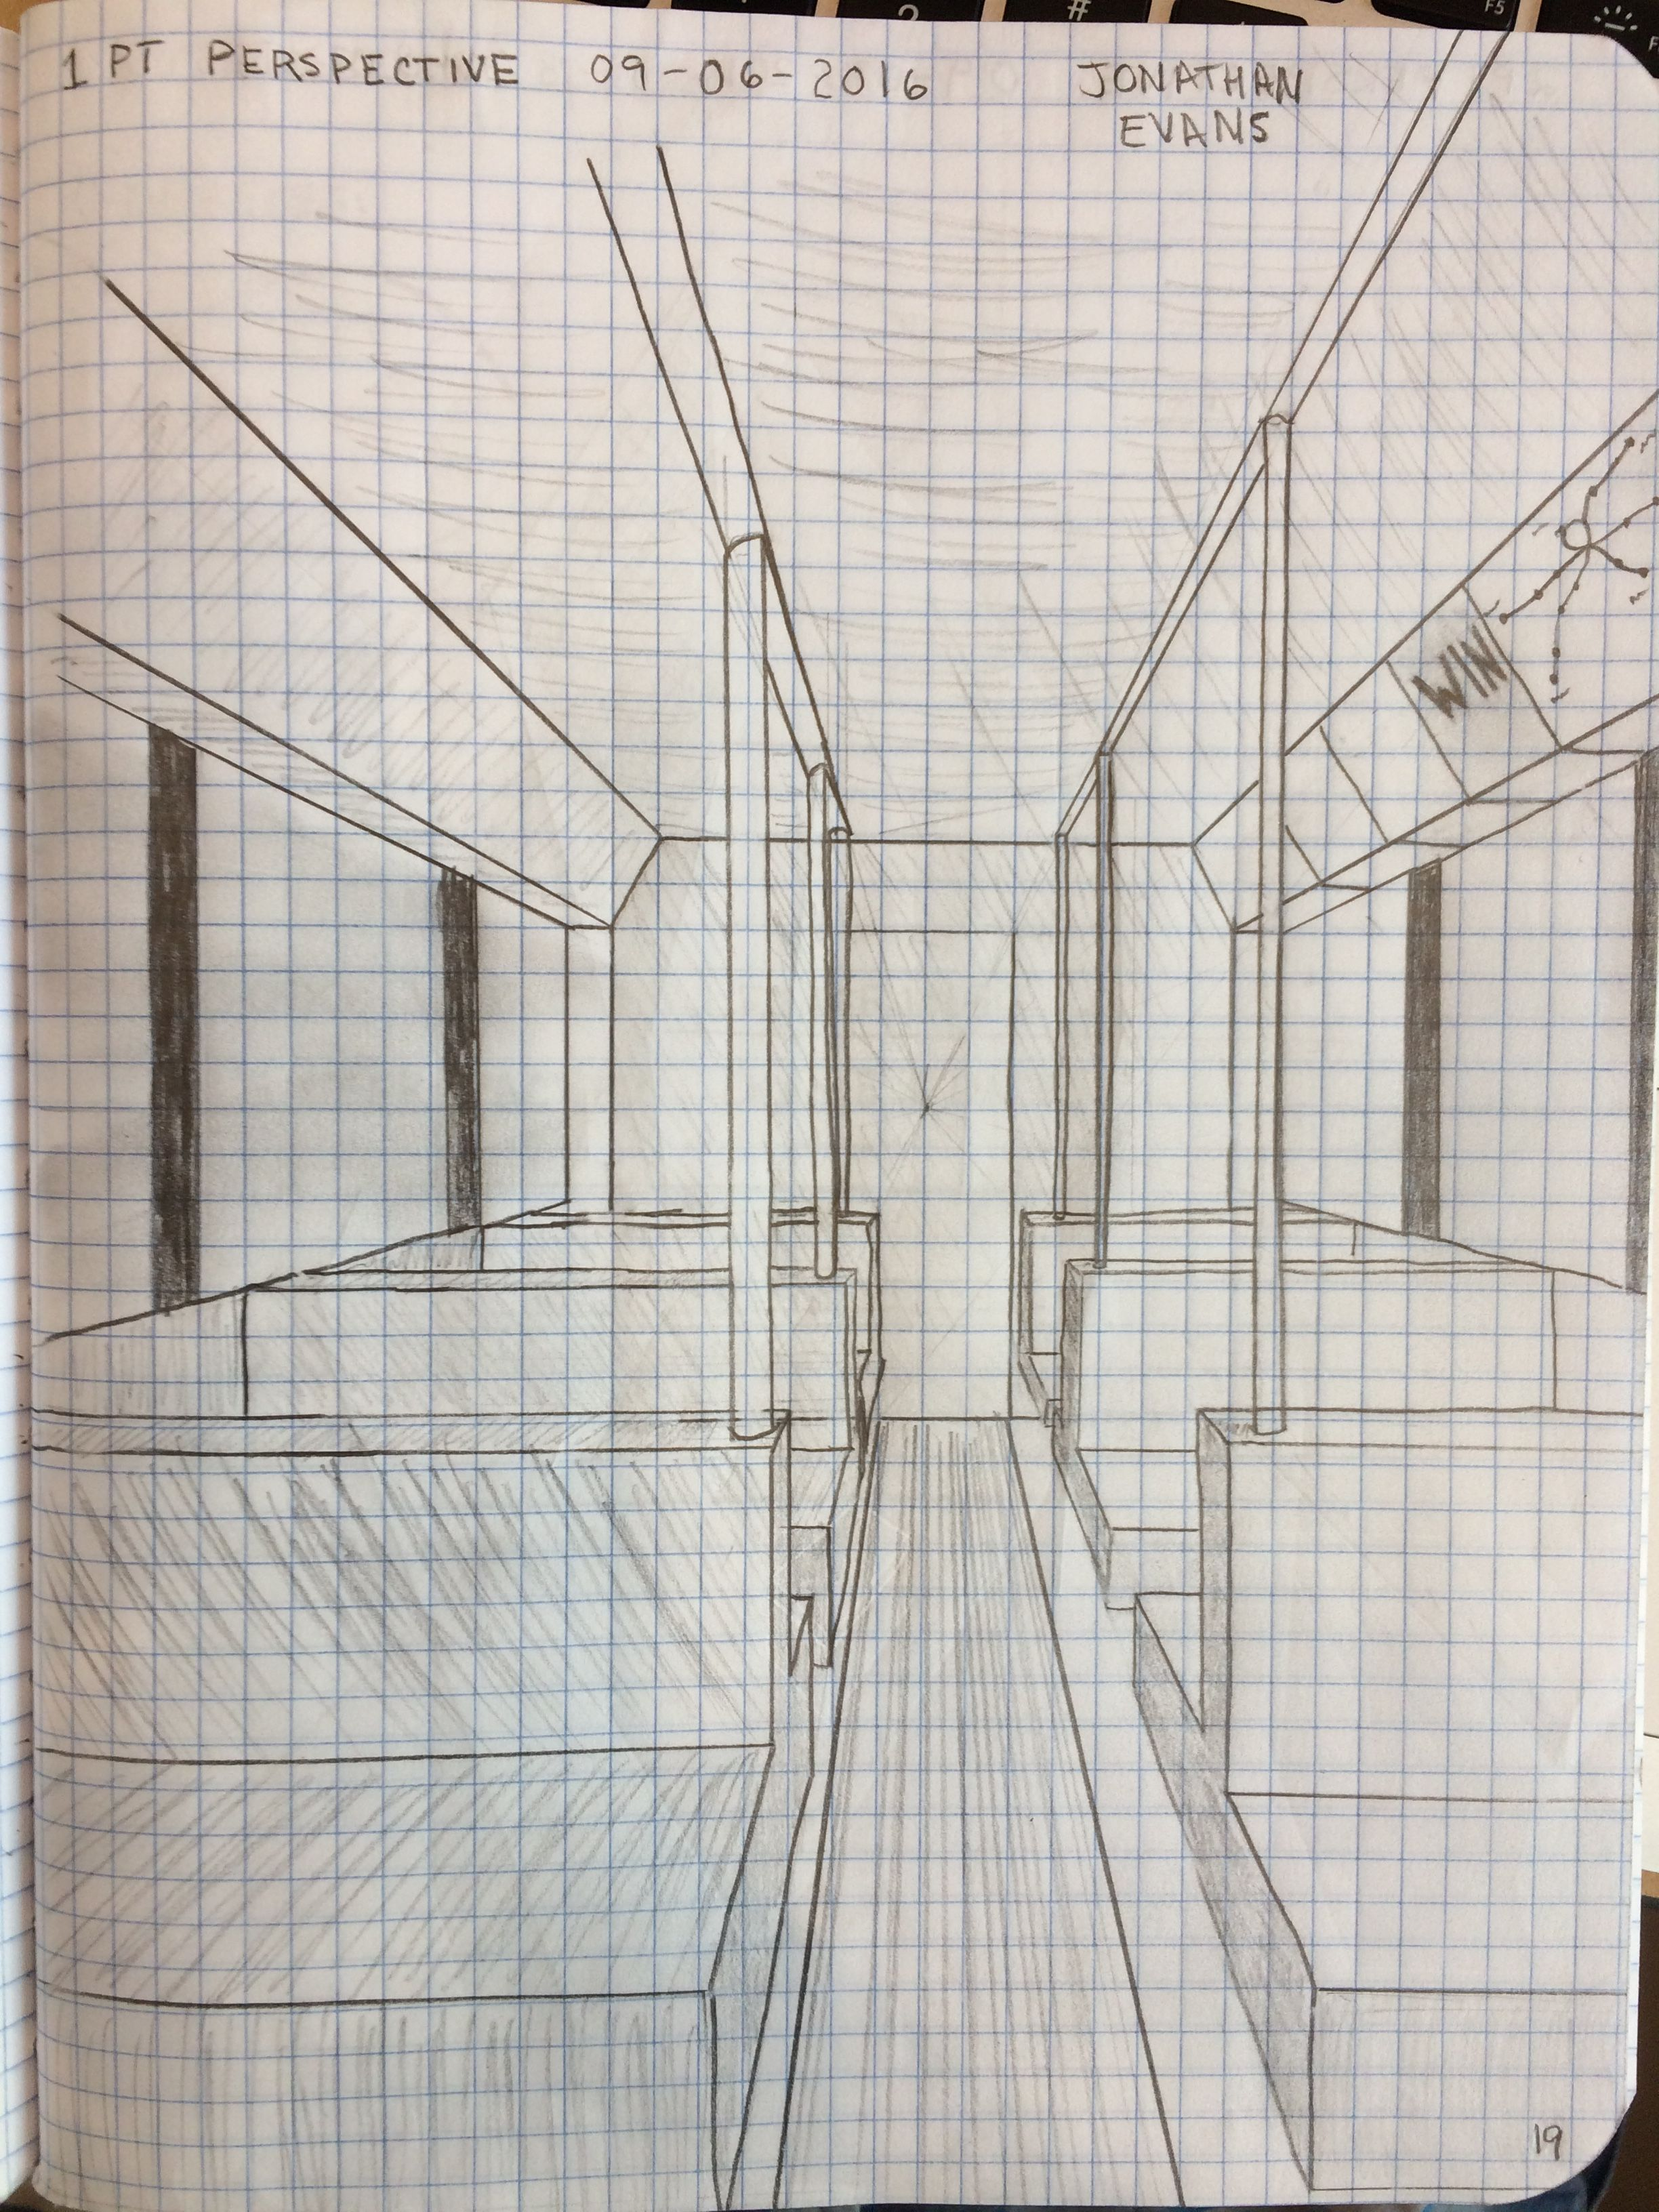
\includegraphics[width=160mm]{resources/light-rail-sketch.jpg}
    \caption{Sketch of Inside of Light Rail}
\end{figure}

\begin{figure}[H]
    \centering
    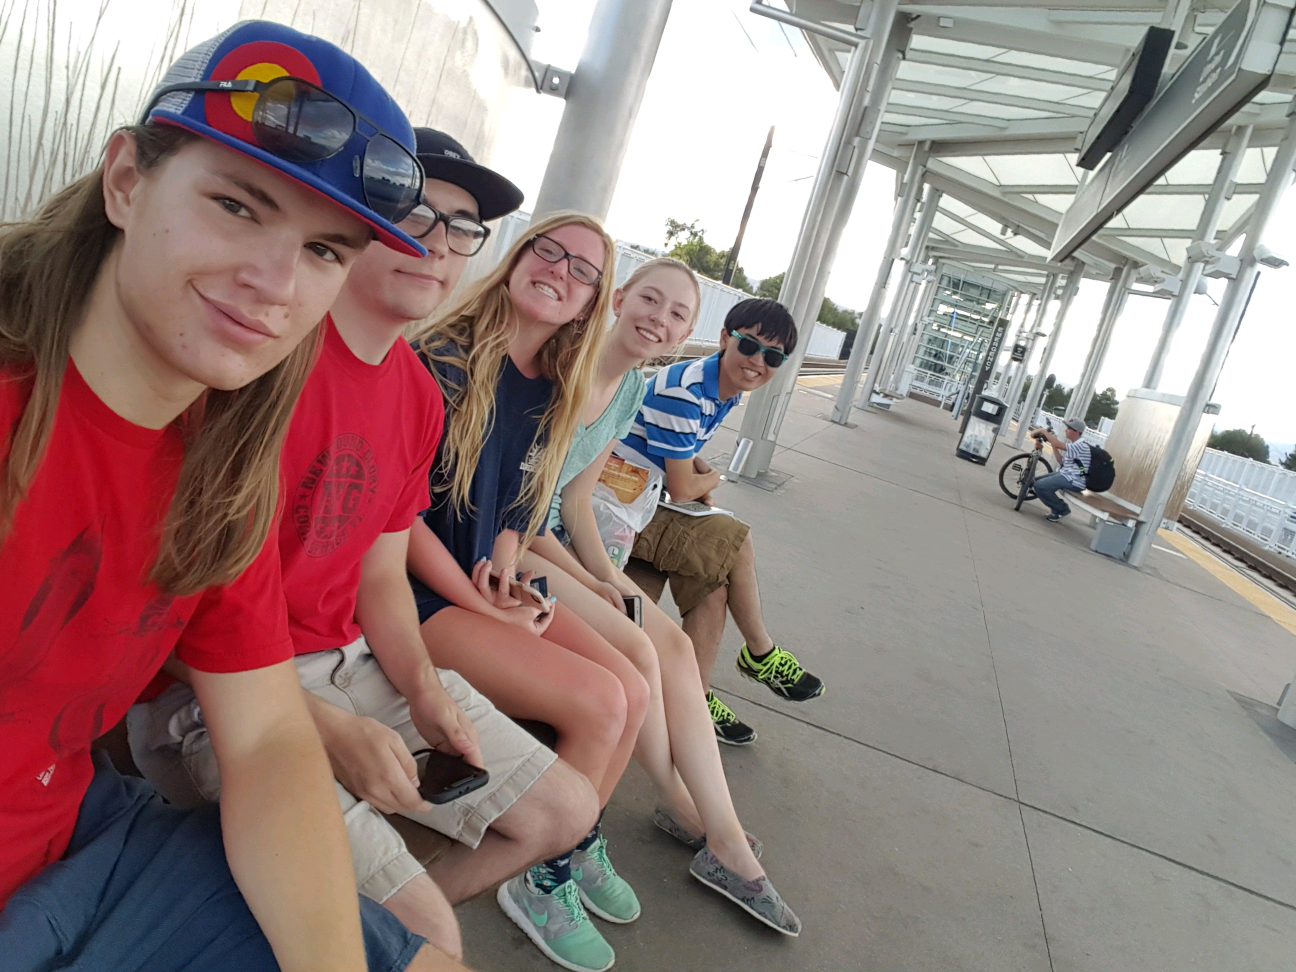
\includegraphics[width=110mm]{resources/team.png}
    \caption{Our team waiting for the next Light Rail train to come}
\end{figure}

\begin{figure}[H]
    \centering
    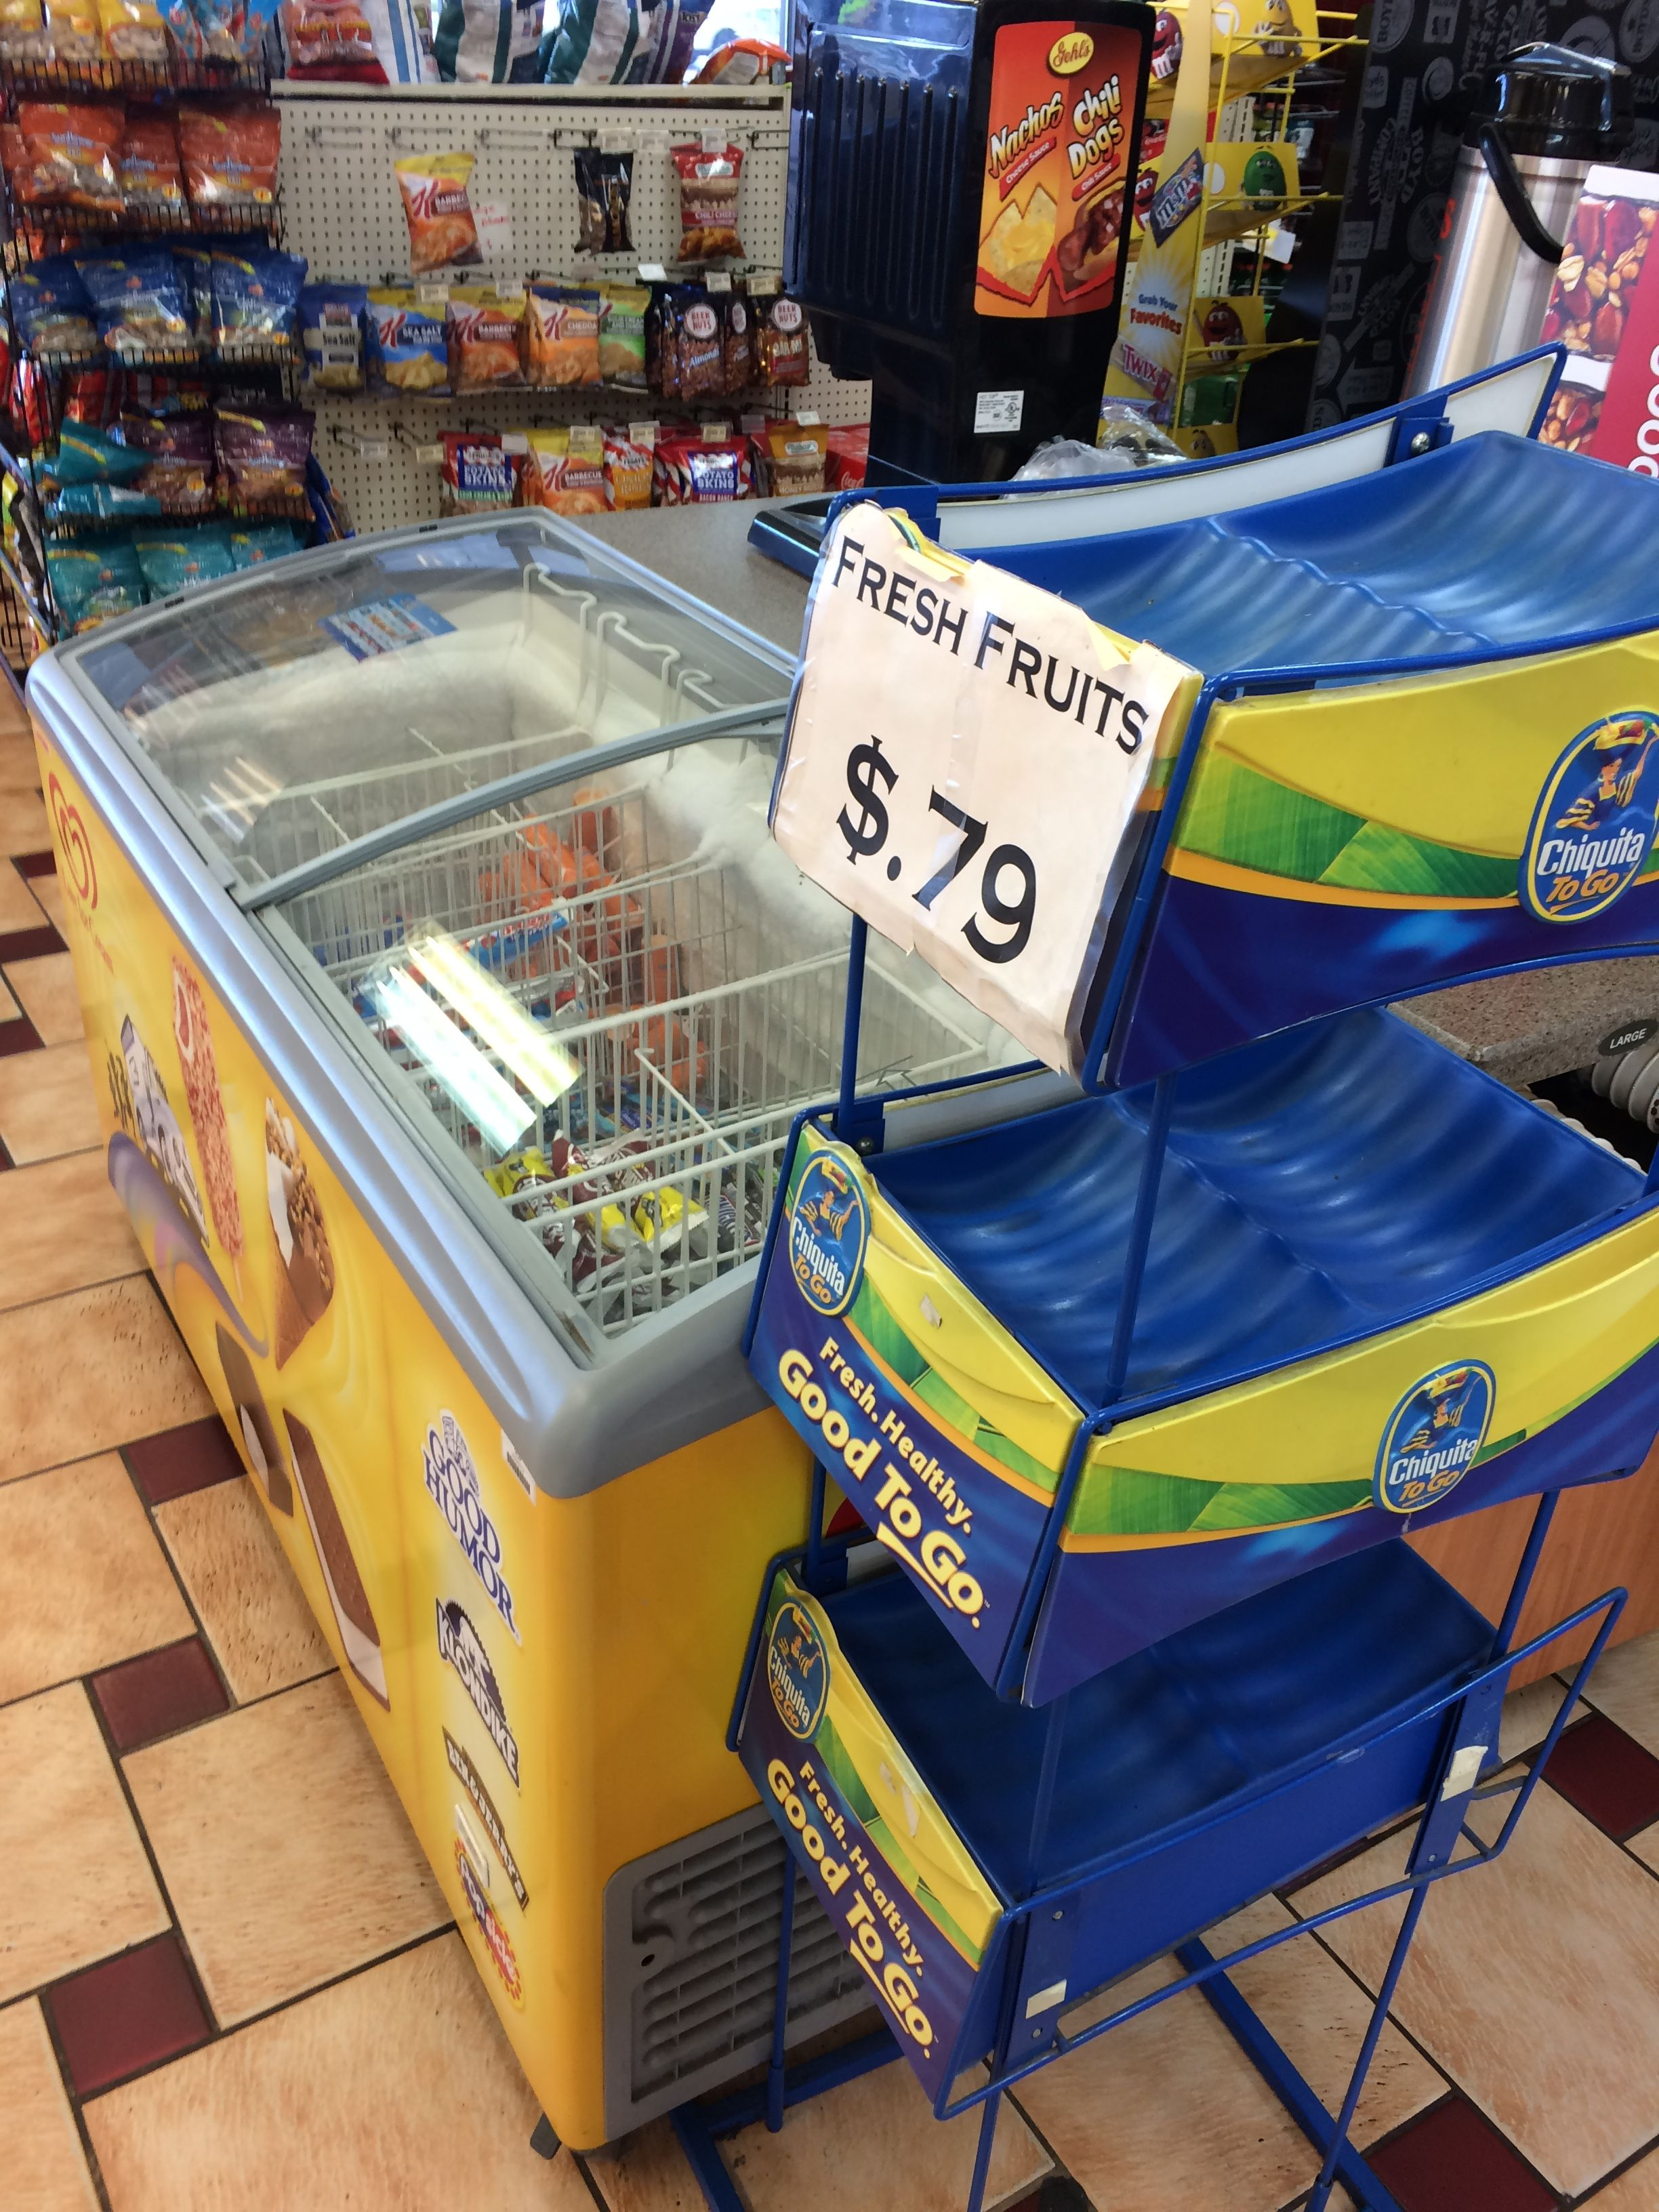
\includegraphics[width=80mm]{resources/empty-banana-stand.jpg}
    \caption{The banana stand was empty but the ice cream freezer was not}
\end{figure}

\begin{figure}[H]
    \centering
    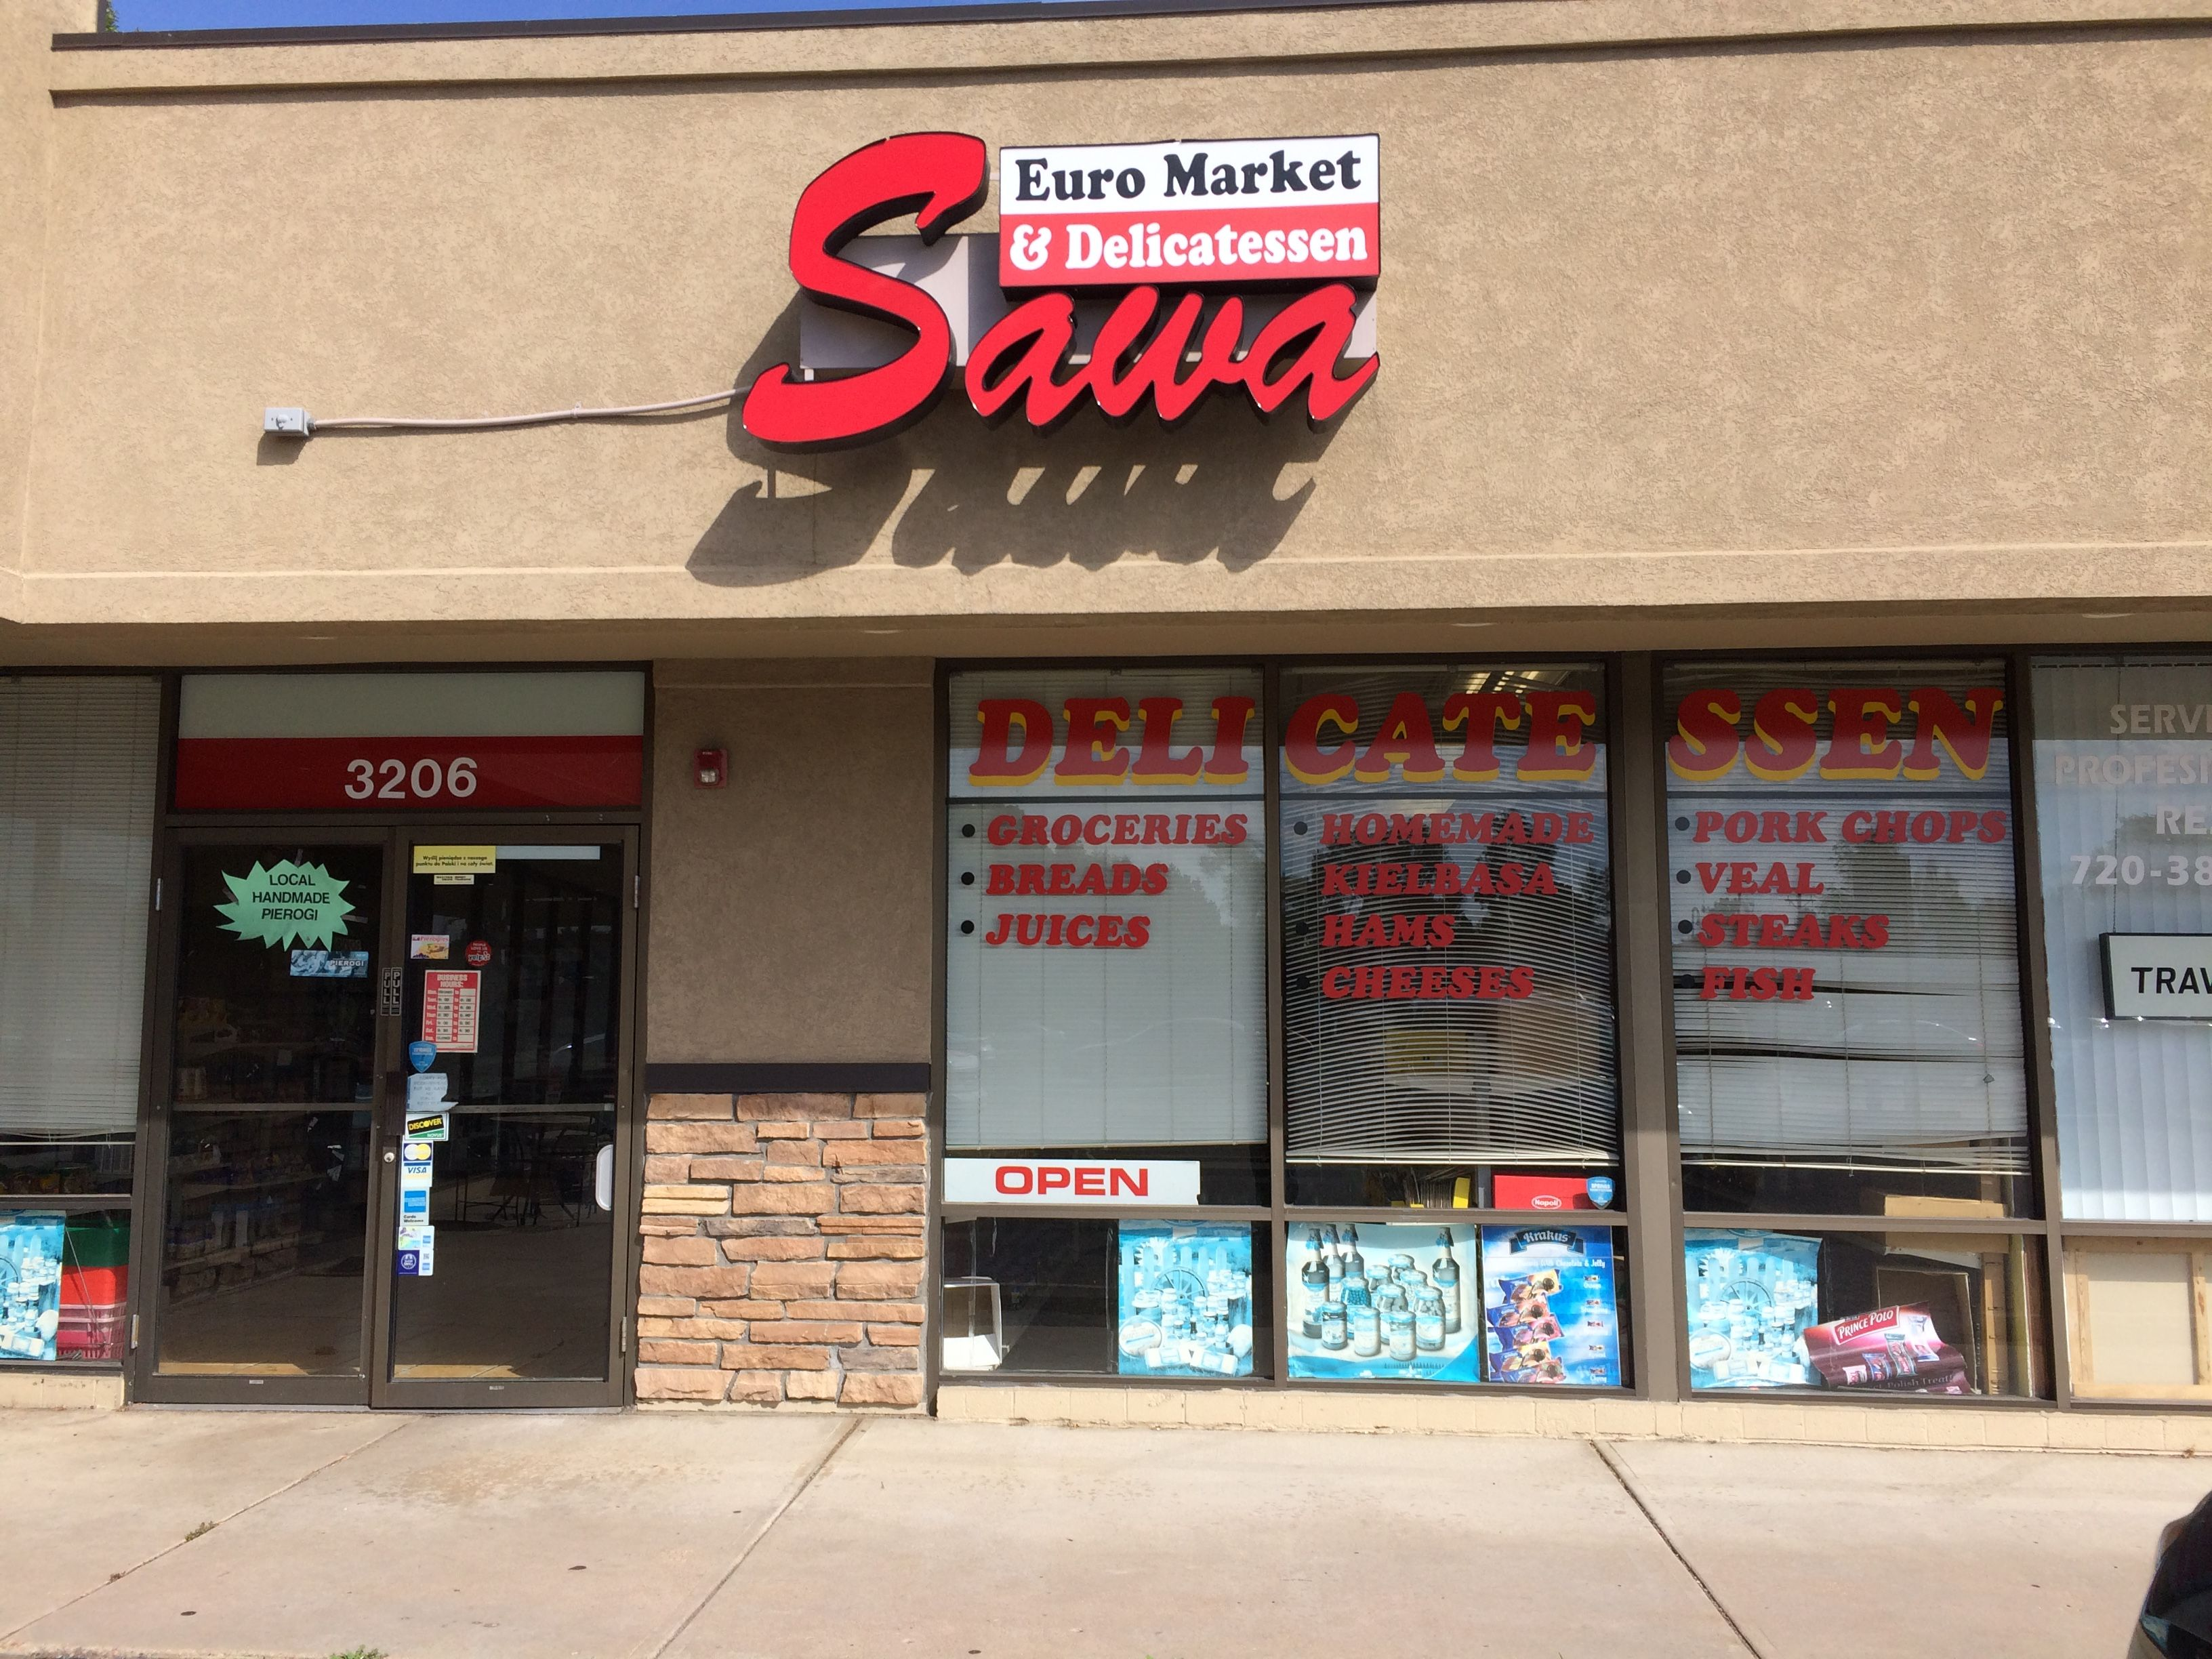
\includegraphics[width=100mm]{resources/delicatessen.jpg}
    \caption{The Euro Market Delicatessen on Wadsworth and 32nd}
\end{figure}

\begin{figure}[H]
    \centering
    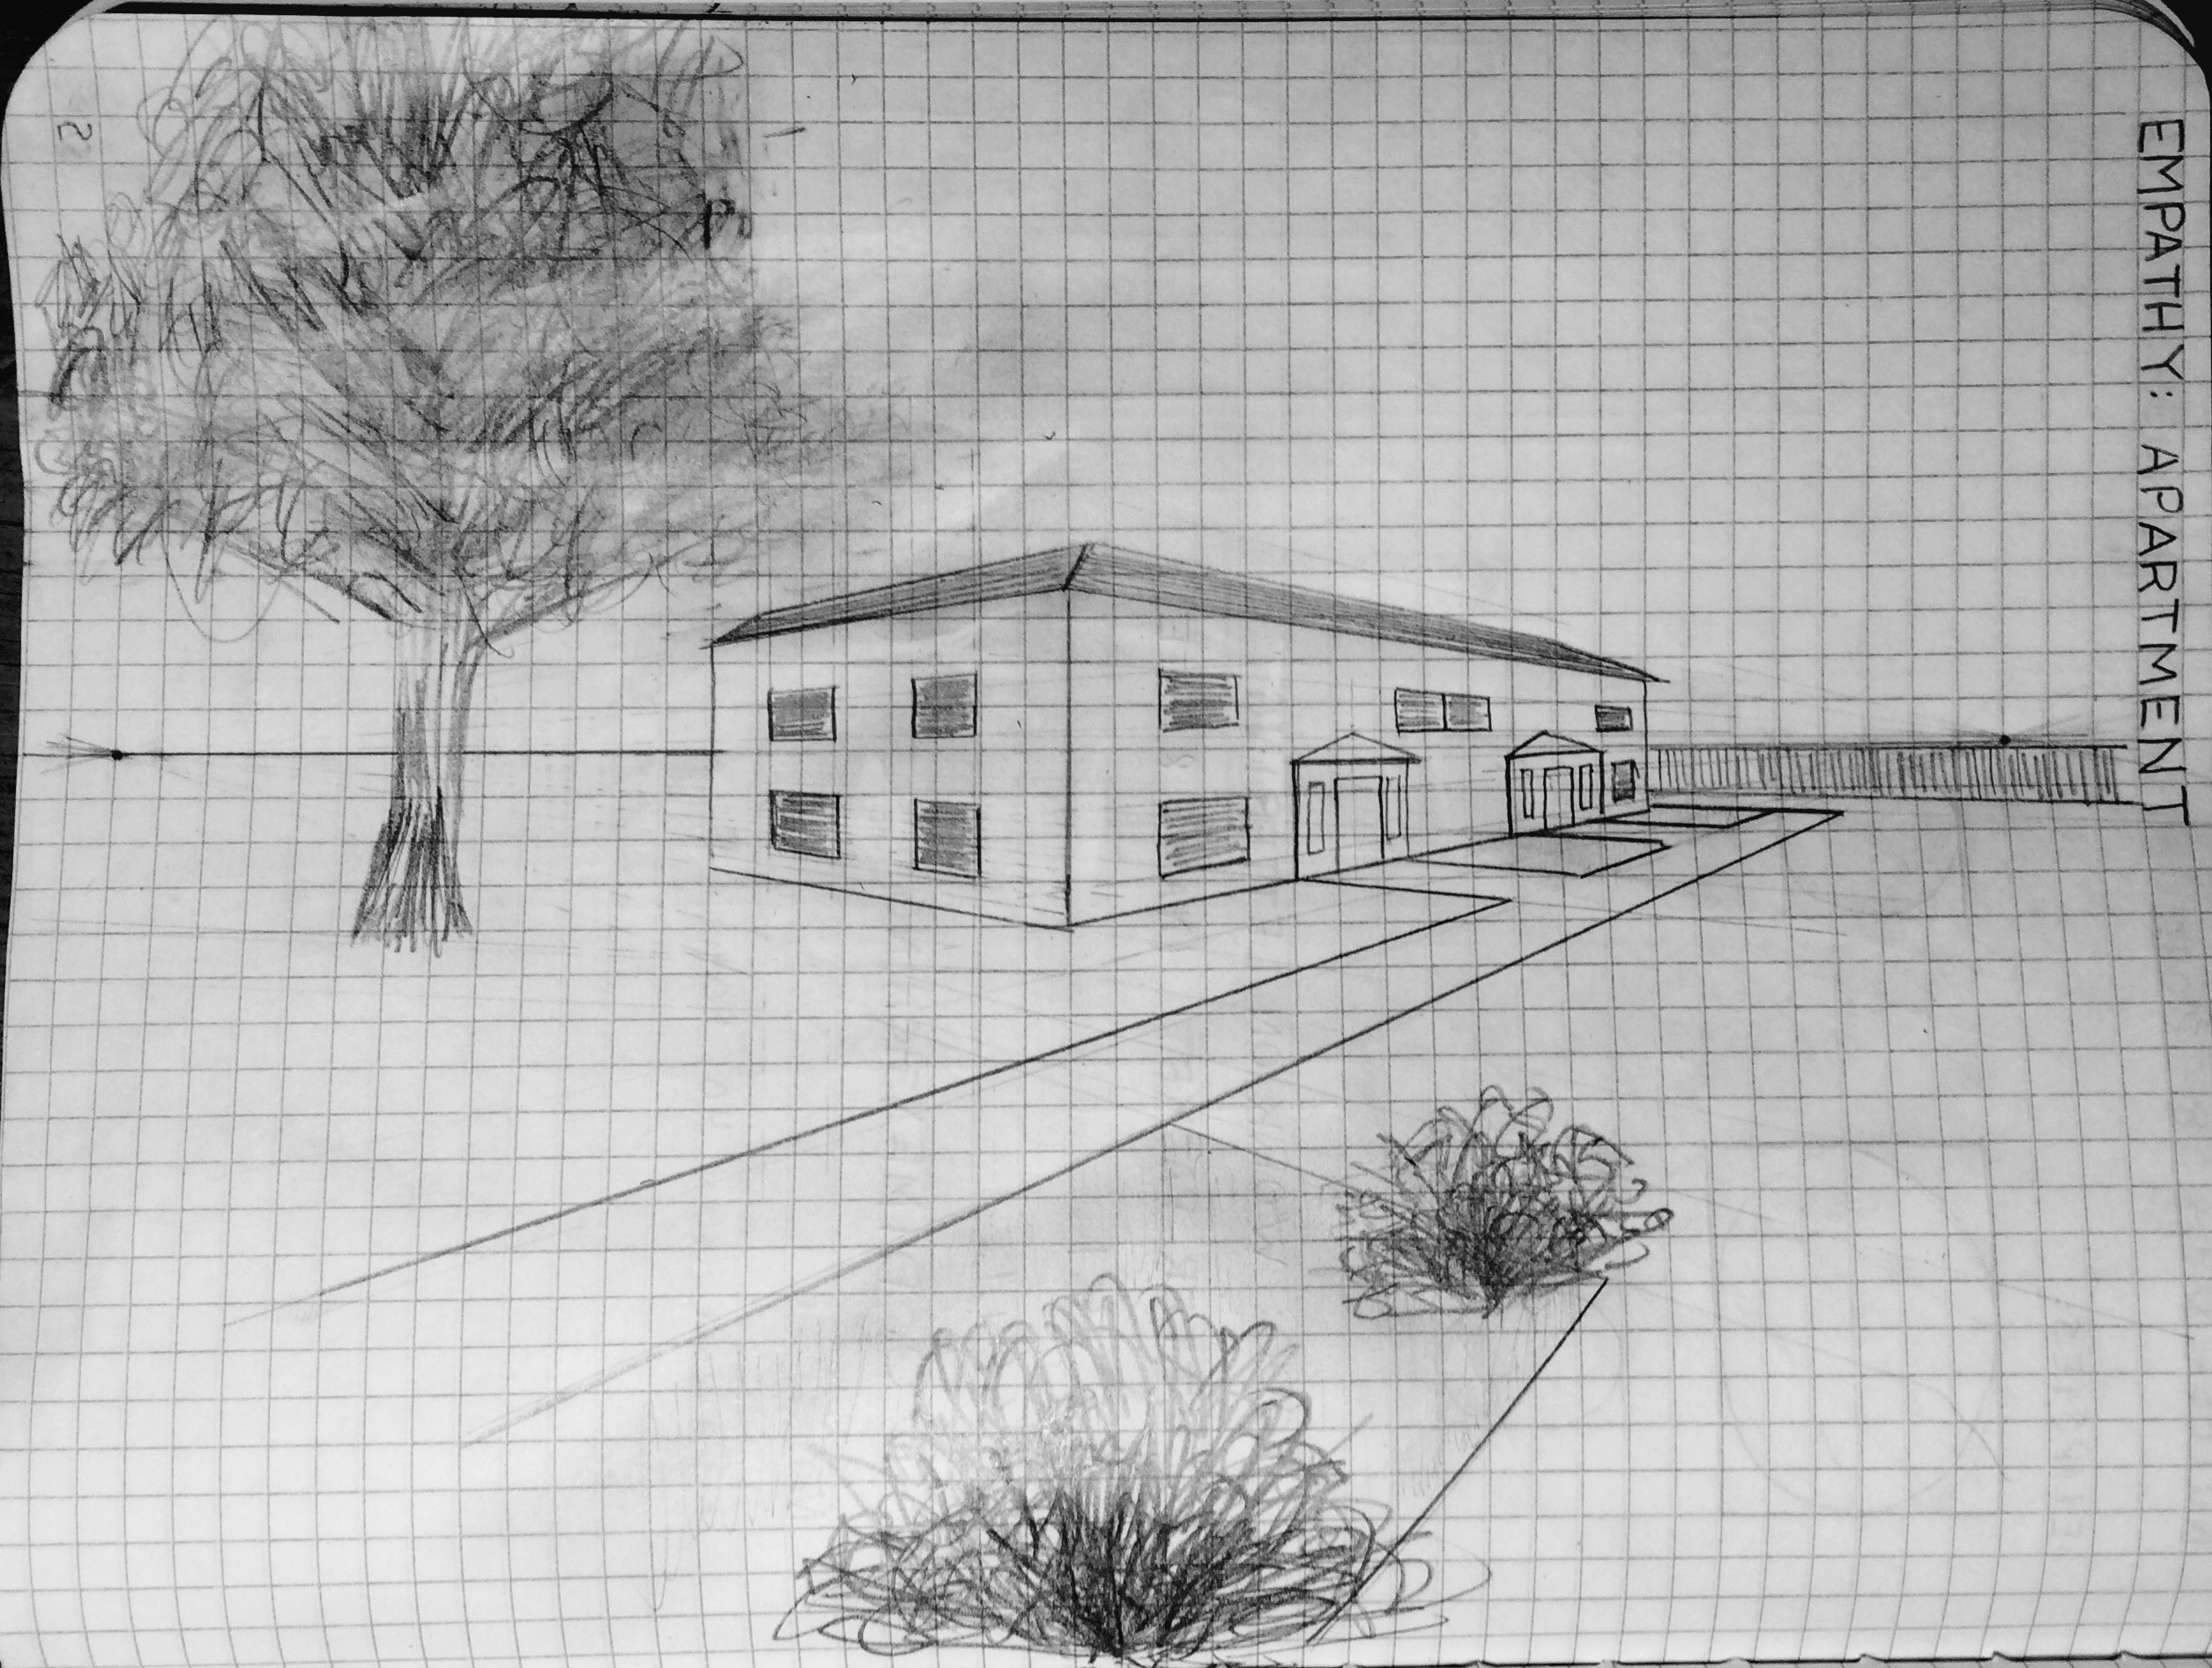
\includegraphics[width=160mm]{resources/apartment.jpg}
    \caption{Sketch of the inside of a Light Rail train}
\end{figure}

\pagebreak
\begin{thebibliography}{9}
    \bibitem{usda-snap}
    United States Department of Agriculture (2016).
    \textit{Supplemental Nutrition Assistance Program (SNAP)} [Online].
    Available: \url{http://www.fns.usda.gov/snap/supplemental-nutrition-assistance-program-snap}.
    [Accessed 11-Sept-2016].

    \bibitem{myplate}
    United States Department of Agriculture.
    \textit{MyPlate} [Online].
    Available: \url{https://www.choosemyplate.gov/}.
    [Accessed 15-Sept-2016]

    \bibitem{fep}
    Food Empowerment Project (2016).
    \textit{Food Deserts} [Online].
    Available: \url{http://www.foodispower.org/fooddeserts}.
    [Accessed 14-Sept-2016]

    \bibitem{cdc}
    Centers for Disease Control and Prevention (2012).
    \textit{A Look Inside Food Deserts} [Online].
    Available: \url{http://www.cdc.gov/features/FoodDeserts/index.html}.
    [Accessed 11-Sept-2016].

    \bibitem{usda-access}
    United States Department of Agriculture Economic Research Service (2009).
    \textit{Access to Affordable and Nutritious Food: Measuring and Understanding Food Deserts and
    Their Consequences} [Online].
    Available:\url{http://www.ers.usda.gov/media/242675/ap036_1_.pdf}.
    [Accessed 14-Sept-2016]

    \bibitem{cbpp}
    Center of Budget and Policy Priorities (2015).
    \textit{A Quick Guide to SNAP Eligibility and Benefits} [Online].
    Available: \url{http://www.cbpp.org/research/a-quick-guide-to-snap-eligibility-and-benefits}.
    [Accessed 11-Sept-2016].

    \bibitem{gallagher}
    Mari Gallagher Research and Consulting Group (2014).
    \textit{Food Desert Balance Community Fact Sheet} [Oneline].
    Available:
    \url{http://www.marigallagher.com/site_media/dynamic/project_files/Food-Desert-and-Food-Balance-Fact-Sheet.pdf}.
    [Accessed 12-Sept-2016].

\end{thebibliography}
\end{document}
